\documentclass{article} % For LaTeX2e
\usepackage{nips14submit_e,times}
\usepackage{hyperref}
\usepackage{url, amsmath, booktabs}
\usepackage{amsmath,amsfonts,amssymb}
\usepackage{float}
\usepackage{wrapfig}
\usepackage{listings}
\restylefloat{table}

\usepackage{geometry}                		% See geometry.pdf to learn the layout options. There are lots.
\geometry{letterpaper}                   		% ... or a4paper or a5paper or ... 
%\geometry{landscape}                		% Activate for for rotated page geometry
%\usepackage[parfill]{parskip}    		% Activate to begin paragraphs with an empty line rather than an indent
\usepackage{graphicx}				% Use pdf, png, jpg, or eps§ with pdflatex; use eps in DVI mode
								% TeX will automatically convert eps --> pdf in pdflatex	
								
\DeclareMathOperator*{\argmin}{arg\,min}
%\usepackage{amssymb}

\title{Amazon Product Recommendations Using Collaborative Filtering and Natural Language Processing  }

\author{
Nikhil Aourpally \\
\texttt{Nikhil.Aourpally@asu.edu} \\
\And
Anthony Helmstetter \\
\texttt{anthony.helmstetter@asu.edu} \\
\And
Prajwal Paudyal \\
\texttt{ppaudyal@asu.edu} \\
\And
Anirudh Som \\
\texttt{Anirudh.Som@asu.edu} \\
}
%\date{}							% Activate to display a given date or no date



\nipsfinalcopy

\begin{document}

\maketitle

\begin{abstract}
In this project we implemented a Recommender System to provide item suggestions based on Amazon user ratings and review text for the Amazon Instant Video platform. The Recommender System was implemented using collaborative filtering. To increase recommendation accuracy, we performed natural language processing on user written reviews to better inform the recommender system of user preferences. We assessed the accuracy of the Recommender System with and without additional textual information contained in user reviews, and investigated ways to further improve the accuracy of the recommender in conjuction with a sentiment analysis of textual reviews. 
\end{abstract}


\section{Introduction}
The range of consumer products and services currently offered has exploded in recent decades. Services like Amazon and Netflix offer an incredible range of products and services, and continue to grow a massive user base. One challenge, a solution of which benefits consumers as well as merchants, is to more quickly, accurately, and efficiently match consumers with desired products. In an age where new data and information are created at an accelerating pace, efficiently filtering out desired information through the undesirable noise is of paramount importance. A recommender system is one such example an information filter. 

Recommender systems attempt to recommend new products to existing users, and perform well when recommended items are indeed desired by user. Personalized recommendations, advertisements, and savings enrich and streamline our online presence.  The main types of recommender systems come in two forms: Content-Based Filters and Collaborative Filtering. Content based filters attempt to match items and users, or users and users, based on content descriptions, keywords, and metadata. This information can be difficult or expensive to obtain, and is a key disadvantage over collaborative filtering. 

Collaborative filtering recommender systems are based on the premise that similar users tend to like similar items, or that similar items tend to be consumed by similar users. As such, collaborative filters are constructed by computing and comparing either user similarity or item similarity. While recommender systems have been well studied in the literature and widely used in practice, we investigated a hybrid recommender system based on natural language processing, inspired by \cite{RecSys}. 

\section{Problem Description}
Our problem involves developing an efficient recommender system to predict, with high accuracy and reliability, the ratings given by users of the Amazon Instant Video service, to videos viewed under that service. To enhance the performance of our recommender system, we will also incorporate additional information derived from text reviews written by users using sentiment analysis and natural language processing, to develop a more accurate metric of user similarity. We will evaluate the performance of our recommender system both with and without the incorporation of additional textual information using NLP and compare the results.

\section{Methodology}
\subsection{Dataset}
The Dataset consists of reviews for movies and television shows available on the Amazon Instant Video service. The data is publically available at \url{https://snap.stanford.edu/data/web-Amazon.html}. The Amazon-Instant-Video subset is 252 MB and consists of 717,651 reviews across 312929 unique users and 22190 unique movies. A typical entry is shown below. 

\begin{verbatim}
product/productId: B002BNZ2XE
product/title: Amazon.com: Moving Target (1988): Jason Bateman, John Glover, 
Jack Wagner, Chynna Phillips: Amazon Instant Video
product/price: 0.00
review/userId: AZVY9Y3A0YU1I
review/profileName: Willard R. Stephen
review/helpfulness: 1/1
review/score: 4.0
review/time: 1277424000
review/summary: Moving Target
review/text: I found this to be an intrieging suspense thriller with a 
minimum of violence and a happy ending. This is a rare combination in 
recent releases. I found it well excepted and enjoyed by teen age 
audiences.
\end{verbatim}

The features of interest in the recommender system will be productId, userId, score, revuew summary, and review text.  The score or rating of a review is an integer value between 1 and 5 inclusive. The review text consists of natural language text of variable length.

\subsection{Preliminary Neighborhood Methods}
Our initial goal was to establish a baseline recommender system without incoporating a natural language processing component. To that end, and following \cite{WBKNN2013} we first explored neighborhood based collaborative filtering methods determined by user similarity. Using a smaller, more manageable subset of the the Amazon Instant Video dataset we computed the similarity between each pair of users. To calculate the similarity between users $u$ and $v$, we first take the intersection of all movies rated by both $u$ and $v$ and create ratings vectors $r_u$ and $r_v$ whose elements consist of the explicit ratings each user, across common movies in the shared intersection. Similarity between users was then calculated by computing the Pearson correlation coefficient between users. 

After all pairwise similarity measures between users were calculated, recommendations for user $u$ could be found by selecting the $k$ most similar users. The predicted rating for a particular movie $i$, previously unrated by user $u$ is then calculated by a weighted combination of the $k$ most similar users' rating of movie $i$.

Due to the fact that a large number of users rated very few movies, or variance between a specific users ratings was so low, the Pearson correlation coefficient proved to be unreliable as a measure of similarity. As the full Amazon Instant Video Set consisted of approximately 312,929 unique users, computing the similarity matrix would require many billions of similarity function calls to compute the Pearson correlation coefficients. Additionally, it was computationally intensive to calculate the intersection of rated items between each pair of user. Procedures to parallelize these calcuations were infeasible, and we explored other options such as matrix mactorization methods. 

\subsection{Matrix Factorization Methods}
Matrix factorization methods offer many advatanges over neighborhood methods, including speed, paralellization, accuracy, and explanatory power. To build a recommender system based on matrix factorization, we transormed a flat list of movie ratings seen in the table on the left, below, into an $m \times n$ matrix depicted below on the right.

% \begin{wraptable}{r}{5.5cm}
% \begin{table}[H]
\begin{figure}[H]
  \caption{Representations of user-item ratings}
  \centering



\begin{center}
\begin{tabular}{l c c} 
\toprule 
UserId & MovieId & Rating \\ 
\midrule % In-table horizontal line
1 & 1 & 5 \\ 
1 & 4 & 2 \\ 
2 & 1 & 4 \\ 
2 & 2 & 3 \\ 
3 & 5 & 1 \\ 
4 & 2 & 1 \\ 
4 & 5 & 4 \\
\vdots  & \vdots & \vdots \\ 
\bottomrule % Bottom horizontal line
\end{tabular}
\quad \quad \quad
% \caption{User-Movie Ratings List} 
% \end{table}
% \end{wraptable}
% \begin{table}[H]
% \begin{center}
\begin{tabular}{c c c c c c c} 
\toprule 
& \multicolumn{5}{c}{MovieId} \\ 
% \cmidrule(l){2-6} 
UserId & 1 & 2 & 3 & 4 & 5 & \dots \\ 
\midrule 
1 & 5 & 0 & 0 & 2 & 0 & \dots\\ 
2 & 4 & 3 & 0 & 0 & 0 & \dots\\ 
3 & 0 & 0 & 0 & 0 & 1 & \dots\\ 
4 & 0 & 1 & 0 & 0 & 4 & \dots\\ 
5 & 5 & 4 & 0 & 0 & 3 & \dots\\ 
6 & 0 & 3 & 2 & 3 & 0 & \dots\\ 
\vdots & \vdots & \vdots  & \vdots  & \vdots & \vdots & $\ddots$ \\ 
\bottomrule 
\end{tabular}
\end{center}
% \caption{User-Movie Ratings Matrix} 
% \end{table}
\end{figure}

The movie rating matrix, $R \in \mathbb{R}^{m \times n}$ has rows corresponding to users, columns correpsonding to movies, where entries $r_{ui}$ give the rating on a 1-5 scale given by user $u$ to movie $i$. This matrix is extremely incomplete, and provides the rationale for constructing a recommender system in the first place. The resulting recommender system attempts to `fill in` the missing entries, while preserving as much as possible the known interactions between users and movies present in the dataset. All ratings for which we have no data are given a value of 0, resulting in an extremely sparse matrix. 

The goal of a matrix factorization recommender is to discover the matrices $P \in \mathbb{R}^{m \times k}$ and $Q \in \mathbb{R}^{k \times n}$ such that $R \approx PQ$. That is, we wish to minimize the norm difference between the known rating $r_{ui}$ and the predicted rating $\hat r_{ui}$ where the predicted rating is given by $\hat r_{ui} = q_i^\intercal p_u$ with $q_i$ and $p_u$ the $i$th column and $u$th row of $Q$ and $P$ respectively. The parameter $k$ determines the effective rank of the matrix factors with $k \ll m,n$. The value of $k$ determines the dimension of the lower dimensional subspace of latent features both in user space and item space that best retain the interactions between users and items. The vector $p_u \in \mathbb{R}^{1 \times k}$ measures the extent to which user $u$ possesses the $k$ latent user features, while the vector $q_i \in \mathbb{R}^{k \times 1}$ measures the extent to which item $i$ possesses the $k$ latent item features \cite{ATTPaper2009}. The interaction between these two vectors, and the predicted rating $\hat r_{ui}$ is given by the inner product of the two feature vectors. The factorization is presented visually below:

\[
  \stackrel{\stackrel{\mbox{rating}}{\mbox{matrix}}}{%
    \begin{bmatrix}
    r_{11} & r_{12} & \cdots & r_{1N} \\
    r_{21} & r_{22} & \cdots & r_{2N} \\
    \vdots & \vdots & \ddots & \vdots \\
    r_{M1} & r_{M2} & \cdots & r_{MN}
    \end{bmatrix}%
  }\ = 
  \stackrel{\stackrel{\mbox{user}}{\mbox{features}}}{%
    \begin{bmatrix}
    p_{11} & p_{12} & \cdots & p_{1K} \\
    p_{21} & p_{22} & \cdots & p_{2K} \\
    \vdots & \vdots & \ddots & \vdots \\
    \vdots & \vdots & \ddots & \vdots \\
    \vdots & \vdots & \ddots & \vdots \\
    \vdots & \vdots & \ddots & \vdots \\
    p_{M1} & p_{M2} & \cdots & p_{MK}
    \end{bmatrix}%
  }\ \quad
  \stackrel{\stackrel{\mbox{item}}{\mbox{features}}}{%
    \begin{bmatrix}
    q_{11} & q_{12} & \cdots & \cdots & \cdots & q_{1N} \\
    q_{21} & q_{22} & \cdots & \cdots & \cdots & q_{2N} \\
    \vdots & \vdots & \ddots & \cdots & \cdots & \vdots \\
    q_{M1} & q_{K2} & \cdots & \cdots & \cdots & q_{KN}
    \end{bmatrix}%
   }
\]
We wish to minimize the squared difference between observed ratings and predicted ratings. Let $\kappa$ be the set of ordered pairs $(u,i)$ for which we have observed ratings between user $u$ and item $i$. To avoid overfitting the training data, we introduce a regularization parameter $\lambda$ to balance the norm of the factorization vectors $p$ and $q$ against the square of the ratings residuals. $P$ and $Q$ then solve the regularized least squares formulation:

\begin{equation}
    (Q, P) = \argmin_{q, p} \sum_{i,u \in \kappa} (r_{ui}-q_i^\intercal p_u)^2 + \lambda( \|q\|^2 + \|p\|^2)
\end{equation}

As both $p_u$ and $q_i$  are unknown there is no closed form solution that minimizes the above functional. To compute the desired factorization we use an Alternating Least Squares approach. In the iterative ALS approach we fix $p_u$ and minimize the objective function with respect to the $q_i$. Then we fix $q_i$ and minimize the objective funcion with respect to $p_u$, alternating as we proceed. Following the work of \cite{Yeung:2010:Online}, we are then minimizing the pair of equations, each with respect to one variable: 
\[ J(p_u) = (r_u - p_u Q) W_u (r_u - p_u Q)^T + \lambda p_u p_u^T \] 
\[ J(q_i) = (r_i - P q_i) W_i (r_i - P q_i)^T + \lambda q_i q_i^T \]
with the binary diagonal weighting matrices $W_u$ and $W_i$ 
\[
   w_{ui} = \left\{
     \begin{array}{lll}
       1 &: &\text{user } u \text{ rated movie } i \\
       0 &: &\text{else}
     \end{array}
   \right.
\]
The original minimization problem is over the sum of $(u,i) \in \kappa$, but with the above weighting matrices, the alternating least squares solution can be found over all $(u,i)$, allowing the algorithm to act on entire vectors as opposied to a sparse set of matrix entries. The minimization of the above equations has closed formed solutions
\[ p_u = (Q .^* W_u Q^T + \lambda I)^{-1} Q W_u r_u \] 
\[ q_i = (P^T .^* W_i P + \lambda I)^{-1} P^T W_i r_i \] 

To procced with ALS, we assign $p_u$ a random initial value, and use the closed form solution to the regularized least squares problem in one variable, to calculate $q_i$. With $q_i$ fixed, we now compute the updated $p_u$ and continue alternating between the two unknowns until convergence or a maximum number of iterations has been achieved. After a baseline recommender system was developed, we began integrating a natural language component to improve recommender accuracy. 


\subsection{Natural Language Processing}

Most eCommerce retailers provide users an option to leave a review for products they have purchased. These reviews not only provide future users an overview of an item, but they also contain valuable information that the retailer can use. User reviews generally come with a text review. The data that we deal with comes with two sections of text reviews: the review summary and the text review (detailed). While the users provide a numerical review, which is what we base our main recommender system on, it is sufficiently clear that the review texts and summaries also contain some valuable information. We can  leverage this information to give a finer grained score to each review. 

Thinking intuitively, when a person looks at a movie to decide on whether or not to watch it, the recommender that is built on review scores gives some information but it misses out on the details that is contained in the text reviews. The goal behind using NLP in our system is so that we can somehow use this information in the review summary and text to fine-tune the review scores that go into the recommender system. For instance for two reviews that have the same initial rating of 4, one review summary and review text might be very positive, while the other one might be mediocre. We want a movie recommender system that is able to mine the information in the reviews and give a recommendation that is appreciative of this extra information. By incorporating a NLP component to the recommender, we don't restrict users' preferences to be discrete valued integers between 1 and 5; rather the NLP leverages additional information on user preferences to create continuous valued, adjusted ratings based on explicit rating and review text. 

While there are many recommendation systems that exist out there, a novelty of this recommendation system is that it finds a way to incorporate the sentiment information in the reviews that others don't take into consideration. A thing to be noted however is that although we use NLP to fine-tune the recommender, the results are not readily testable since we will ultimately compare against the numeric reviews in the test set, thus we don't expect the NLP system to do better than the base system in that respect. However we do fine tune our NLP system and the combination algorithms such that the overall test error is minimized.  
 
\subsubsection{Stanford NLP.} The first method that we tried was the sentiment Analyzer that is provided by Stanford NLP lab ?. This sentiment analyzer utilizes a 'Semantic Treebank' that includes fine grained sentiment labels for 215,154 phrases in the parse trees of 11,855 sentences. This technique claims to increase the accuracy of predicting-fine grained sentiment labels for all phrases to 80.7 percent. This technique also successfully detects negation in a sentence which is very important for sentiment analysis on movie reviews. After compilation of the NLP files, we get a 'pipeline' which takes a single sentence at a time and gives back a score that is between 0 and 4 which is convenient as it allows us to scale the output and combine it directly with our base recommender system. A typical semantic analyzer has the form

\begin{lstlisting}[language=bash]
java -cp "*" -Xmx2g edu.stanford.nlp.pipeline.StanfordCoreNLP 
-annotators tokenize,ssplit,pos,lemma,ner,parse,dcoref 
-file input.txt
\end{lstlisting}

 Our recommender system would first get a sentiment value for the Review Summary section, then it would parse the Review Text section into individual sentences, get a sentiment value for each of those sections and then combine them and normalize it. We gave a slightly higher score to the Review Summary section than the review score section based on the formula:
\[
\frac{1.2 \times \text{Review Summary Score} + \text{Review Text Score}}{4.4}
\]
We more heavily weighted the Review Summary over the Review Text as we found the Review Summary more directly and succintly expressed the sentiment of the user's preference for the movie, while the review text more often consisted of justification for rating, or an analysis of plot elements pertaining to the movie. 

Although this approach seems to give us good results, we had to abandon it ultimately because it was computationally infeasible and it could not give us results in a timely manner. The system took about 1 second to give a score back for each sentence review. We were processing about 600,000 reviews, which roughly translates to 6 million sentences, which amounts to about 70 days of runtime. On top of that there was the overhead of combination and some isolated cases where the sentence spanned more than 60 words which exponentially increased the processing time. 

\subsubsection{Python TextBlob} The next approach we utilized for natural language processing was TextBlob \cite{TextBlob}. It provides a simple API for diving into common natural language processing (NLP) tasks such as part-of-speech tagging, noun phrase extraction, sentiment analysis, classification, translation, and more. Then we used the sentiment analysis module of this to receive a sentiment score between -1 and 1. The module returned a tuple of the form Sentiment(polarity,subjectivity). The polarity score is a float within the range [-1.0, 1.0]. The subjectivity is a float within the range [0.0, 1.0] where 0.0 is very objective and 1.0 is very subjective. We did not utilize the objectivity score in our NLP processing primarily because we did not want to differentiate between a negative reviews that was very objective vs. one that was subjective. (Example. The movie was awful vs. I felt the movie was awful).  However, after going through several movie reviews, we realized that a good portion of the reviews were plot descriptions and not actual sentiments on the movie. In this light, giving more weight to reviews with higher subjectivity might increase the effectiveness of the sentiment analyzer. Due to time constraints, we were not able to run a detailed test on this aspect and had to set this aside for future work. The TextBlob library uses the PatternAnalyzer software library for sentiment analysis by defaut. We experimented with a Naive Bayes Classifier for sentiment analysis, but again found it computationally infeasible given the size of our data set. We continued to continue using the PatternAnalyzer for all future sentiment analysis. 


As compared to the Stanford NLP processor, the textBlob algorithm was very fast. We used a similar method to parse the Review Summary vs. the Review Text and fed it to the textBlob. We also noticed that this NLP system was able to handle entire paragraphs at a time, which was one of the reasons it was much faster. This algorithm was able to compute the entire training set of close to 600,000 reviews in less than 29 minutes. The result of the analysis was a sentiment score of between -1 and 1. In order to compare the sentiment score of the text reviews to the explicit integer ratings given by the user, we needed to transform the NLP score from [-1, 1] to a 1-5 score. This was acheived by the formula, $\text{Base NLP} = 2 \times \text{NLP} + 3$. This gauranteed NLP scores of -1 and +1 corresponded to a 1 and 5 on the integer scale, respectively. 

\subsubsection{Combination}We noticed that the sentiment scores that were returned was somewhat positively skewed, that is, an overwhelming number of sentiment scores were positive, even in cases where the user explicitly rated the movie as a 1. If we attempted to adjust the explicit ratings with these sentiment scores, we would have effectlively shifted the overall scores upwards instead of just providing a means to differentiate between reviews with the same initial score. As we believe the TextBlob NLP package was reporting positively biased sentiment scores on our data set, we performed a simple mean shift to the NLP scores. For instance, for sentiment scores for movies rated $j$, $j=1...5$, we computed the mean sentiment score over reviews corresponding to a rating of $j$, and subtracted the computed mean from each sentiment score. This made a lot of intuitive sense and also helped us reduce the testing error after we utilized the NLP system. We were then able to transform discrete explicit ratings to sentiment adjusted continous values in which explicit ratings were lowered slightly if the sentiment analysis for that review came back as being more negative than the average sentiment score for movies of the same rating, and adjustments were made proportionally to the difference from the mean sentiment score.

\begin{figure}[H]
  \centering
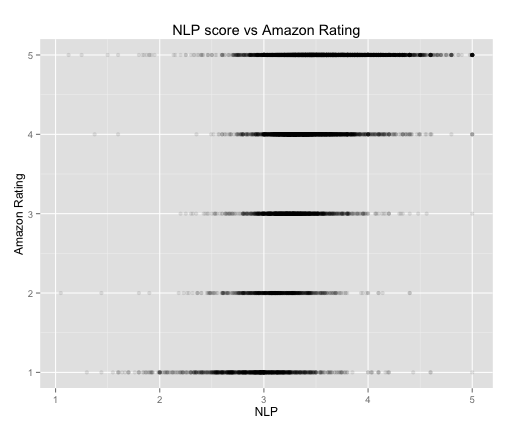
\includegraphics[scale=0.4]{amazon}
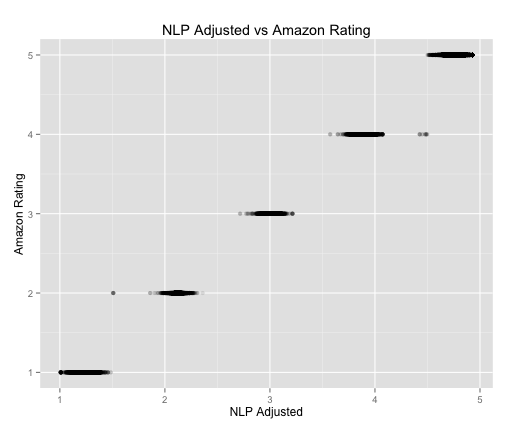
\includegraphics[scale=0.4]{adjusted}
\caption{The figure on the left shows the positive bias in the sentiment scores and the need for mean centering the adjustments. The figure on the right shows the discrete amazon ratings plotted against the continous sentiment adjusted ratings.}
\end{figure}

We then used this shifted NLP scores to adjust the integer ratings according to the formula
\[
\text{Rating Adjusted} = \text{Original Rating} + \alpha \bigg( \frac{\text{Based Shifted NLP} - \text{Original Rating}}{4} \bigg)
\]
The $\alpha$ here is the limiting factor which essentially limits how large of an effect we allow the NLP to have on the adjusted rating. For $\alpha = 0.5$, the NLP portion will be able to adjust the original integer rating by at most 0.5 numeric score i.e. a review of 2 will have an adjusted score of 2 $\pm 0.5$. 

\section{Results}
Parameter optimization was performed using 5-fold cross validation with an additional 15\% of data being held out from cross validation in order to estimate test error. We optimized over four parameters: the rank of the latent features in the matrix factorization, the number of iterations performed in ALS, the regularization parameter $\lambda$, and the NLP combination parameter $\alpha.$ We considered models with rank $k=10,20,40,80$, number of iterations $n=5, 10, 15, 20$, regularization parameter values $lambda$ spaced logarithmically between 10 and .0001, and $alpha = 1, .75, .5$. We obtained optimal model parameters: $r=80$, $n=20$, $\lambda=0.15$. Cross validation for model selection was performed on both the stand-alone recommender system and the recommender system sentiment analyser hybrid. 

\begin{figure}[H]
  \centering
    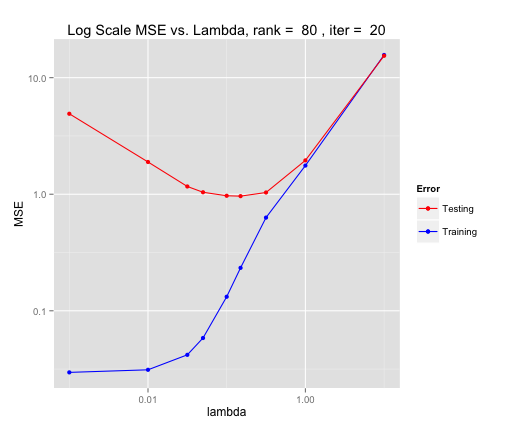
\includegraphics[scale=0.5]{effect_lambda}
     \caption{Bias-Variance Tradeoff}
\end{figure}

Here we see the effect of the regularization parameter on both cross validation testing and training error. Note the iconic U shaped curve highlighting the bias variance trade off. As the $\lambda$ goes to 0, training error goes to 0. Testing error is minimized for $\lambda = .15$.

\begin{figure}[H]
  \centering
    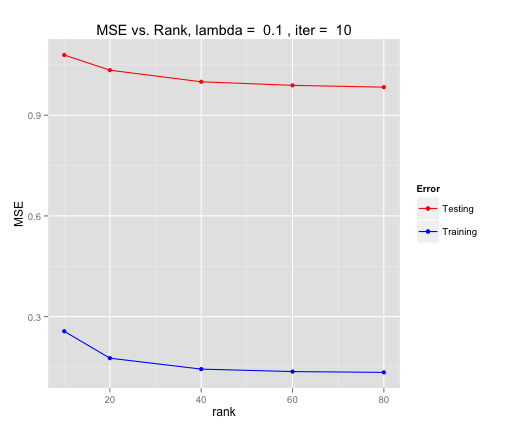
\includegraphics[scale=0.4]{effect_rank}
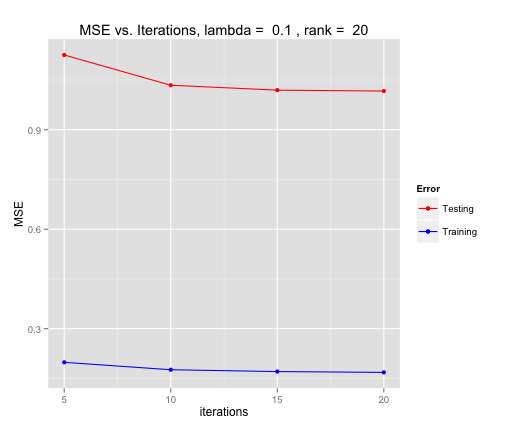
\includegraphics[scale=0.4]{effect_iter}
\caption{Effect of parameter values on mean squared error}
\end{figure}

Here we see the effect of changing rank and the number of iterations in ALS. Both results are expected as we see decreasing testing and training error as we allow a greater of number of latent features to be discovered by the matrix factorization. A greater number of iterations corresponds factors given more time to converge towards the true least squares minimizer. To reiterate, two recommender systems were built, one on the explicit integer valued user ratings and a second a the sentiment adjusted ratings. It was our belief that finer grained, continous valued ratings would allow a richer set of features to be unconvered by the matrix factorizarion. Whereas a user might explicitly rate many movies as the same, there is an inherent ranking and preference held by the user on the equally rated movie, and this information might be accessible by analysing textual reviews. 

The integer trained recommender system had a mean squared error of 0.23 on the training test, and 0.962 on the final holdout testing set. The sentiment adjusted recommender has similar results. Note that we can't compare the two recommender systems directly, as they were trained to predict different measures. We feel the sentiment adjusted recommender might more accuractly reflect preferences across equally rated movies, but without the data (an ordered ranking of movies by user), we can't verify this claim. 

In an attempt to compare the two recommender directly, we compared their ability to predict integer ratings of movies. That is, both recommenders output continuous values as predictions and given the discrete scale designed by amazon, we rounded the continous predictions to the nearest integer and computed the MSE against the known interger ratings. The baseline recommender system achieved a test MSE of 1.02, while the sentiment adjusted recommender performed slightly worse with a test MSE of 1.04. While still accu`'rate, the sentiment adjusted recommender performed slightly worse than the base recommender. 


\section{Conclusions and Future Work}
Retailers and service providers recommend products to users based on their past preferences. Is it increasingly common to use techniques like Collaborative filtering and content based filtering to provide these recommendations. User/item similarity and matrix factorization are the two widely used Collaborative filtering techniques. Although user similarity gives good recommendations we adopted the matrix factorization technique to implement the recommendation system as it was a more compuatationally feasible approch. We attempted to leverage additional information contained in review text to make targeted recommendations. 

There are many opportinuties and paths to improve this work. We can utilize more accurate (and most costly) sentiment analysis tools. We can improve the baseline recommender system by allowing for additional user and movie biases as presented in the literature. Our approach might also see better results in reviews outside of the domain of movies and books. Most of the users in the Amazon Instant Video Dataset that we used decribe the plot of the movie in the review text rather than their opinion about the movie, confounding the sentiment analysis. In all, we have presented a promising investigation of recommender systems, and look forward to improving upon our results. 

\bibliographystyle{plain}
\bibliography{firstDraft}	
\end{document}  